\documentclass[a4paper,10pt]{scrartcl}

\usepackage[utf8]{inputenc}
\usepackage[ngerman]{babel}
\usepackage[T1]{fontenc}
\usepackage{amsmath}
\usepackage[section]{placeins}
\usepackage{graphicx}
\usepackage{esvect}
\usepackage{amssymb}


\title{Praktikum B Vorbereitung zu Versuch "gp"}
\author{Leon Machtl und Raphael Lehner}
\date{9.12.2019}

\begin{document}
	\maketitle
	\tableofcontents
	\newpage
	
	\section{Einleitung zum Versuch}
		Im folgenden Versuch wird das Verhalten von gekoppelten Pendeln genauer betrachtet. Die Oszillation von zwei identischen gekoppelten Pendeln wird vor allem über zwei Begriffe charakterisiert. Die Schwebungsdauer beschreibt das Zeitintervall zwischen zwei Schwingungen eines Pendels mit seiner maximalen Amplitude. Der andere Begriff ist die sogenannte Oszillationsperiode.\\
		Allgemein gehalten lässt sich sagen, dass bei gekoppelten Pendeln die Oszillationsenergie von dem einen Pendel auf das andere übertragen wird. In dem Fall, dass beide Pendel identisch sind und bei Beginn der Oszillation des einen Pendels das andere gerade in Ruhe ist, wird während der Schwingung die Energie des ausgelenkten Pendels vollständig auf das zweite Pendel übertragen, das erste pendel ist dann also in Ruhe, wenn das zweite mit maximaler AMplitude schwingt. Wie oben bereits angesprochen heißt die Zeit zwischen zwei solchen Durchgängen Schwebungsdauer.\\
		Den gesamten Vorgang kann man als Superposition natürlicher Oszillationen betrachten. Folgende natürlichen Oszillationen gibt es:
		\begin{itemize}
			\item Pendel schwingen vollkommen in Phase
				\begin{align*}
				\phi_{1}=\phi_{2}=\phi
				\end{align*}
			\item Pendel schwingen vollkommen außer Phase
				\begin{align*}
				\phi_{1}=-\phi_{2}=\phi
				\end{align*}
		\end{itemize}
		Im ersten Fall entspricht die Frequenz der Frequenz ungekoppelter Pendel. Im zweiten Fall ist der Kopplungseffekt maximal und die Frequenz ist ebenso maximal.
		
		\subsection{Bewegungsgleichungen}
			\begin{itemize}
				\item Pendelschwingung:\\
				\\
				Es wirke eine zum Auslenkwinkel \(\phi\) proportional rücktreibende Kraft. Dann gilt unter Vernachlässigung der Reibung:
				\begin{align}
				\ddot{\phi}(t)+\omega_{0}^{2}\phi(t)=0
				\end{align}
				wobei \(\omega_{0}\) die Eigenkreisfrequenz bezeichnet. Die allgemeine Lösung lautet dann:
				\begin{align}
				\phi(t)=a\cdot cos(\omega_{0}t)+b\cdot sin(\omega_{0}t)
				\end{align}
				\item Gekoppelte Schwingung:\\
				\\
				Unter der Annahme einer Federkopplung und gleicher Schwingungsdauer beider Pendel, ergeben sich folgende drei Möglichkeiten:
				\begin{itemize}
					\item Gleichsinnige Schwingung (in Phase)\\
					Auslenkung um den gleichen Winkel \(\Psi_{1}(0)=\Psi_{2}(0)\). Die Pendel schwingen parallel nebeneinander. Wenn die Trägheit der feder vernachlässigt wird, wird kein Drehmoment auf die Pendel ausgeübt, somit schwingen sie mit der selben Frequenz \(\omega_{1}=\omega_{2}=\omega_{gl}\).
					\item Gegensinnige Schwingung (gegenphasig)\\
					Auslenkung um den gleichen Winkel in entgegengesetzte Richtung \(\Psi_{1}(0)=-\Psi_{2}(0)\). Verformung der Kopplungsfeder; sie übt also ein Drehmoment auf die Pendel aus. Diese hängen von der Auslenkung der Pendel ab. Solche symmetrische Schwingungen verlaufen mit der Frequenz \(\omega_{1}=\omega_{2}=\omega_{geg}\).
					\item Kopplungsschwingung\\
					Ein Pendel wird um \(\Psi_{1}(0)\neq 0\) ausgelenkt, während das zweite in Ruhe verbleibt. Dann wird das zweite durch das erste zur Schwingung mit wachsender Amplitude angeregt. In diesem Vorgang verliert das erste pendel seine Amplitude nach und nach, bis die Energie komplett auf das pendel übertragen wurde, das zu Beginn in Ruhe verblieb. An diesem Punkt befindet sich nun seinerseits das erste Pendel in Ruhe. Dieser Prozess kehrt sich dann um und wiederholt sich.In diesem Fall, den man auch Schwebungsschwingung nennt, definiert man:
					\begin{itemize}
						\item beide Pendel schwingen ungefähr mit der gleichen Frequenz, während sich die Amplitude ständig ändert \(\omega_{+}\approx \omega_{gl}\approx \omega_{geg}\) 
						\item \(\omega_{-}\) ist die Frequenz, mit der sich die Amplitude der Schwingung ändert (Schwebung)
					\end{itemize}
					Unter Annahme eines symmetrsichen Aufbaus (gleiche Pendellänge, gleiches Trägheitsmoment \(\Theta\), gleiche Winkelrichtgröße \(\tilde{D}\)) und einer linearen Kopplung, folgt für die Drehmomente der Pendel mit Federkonstante \(D\):
					\begin{align}
					M_{1}=-\tilde{D}\cdot \phi_{1}+Dr^{2}(\phi_{2}-\phi_{1})+M_{0}
					\end{align}
					\begin{align}
					M_{2}=-\tilde{D}\cdot \phi_{2}+Dr^{2}(\phi_{2}-\phi_{1})+M_{0}
					\end{align}
					Als Bezugssystem wurden die Lotgeraden verwendet.\\
					\\
					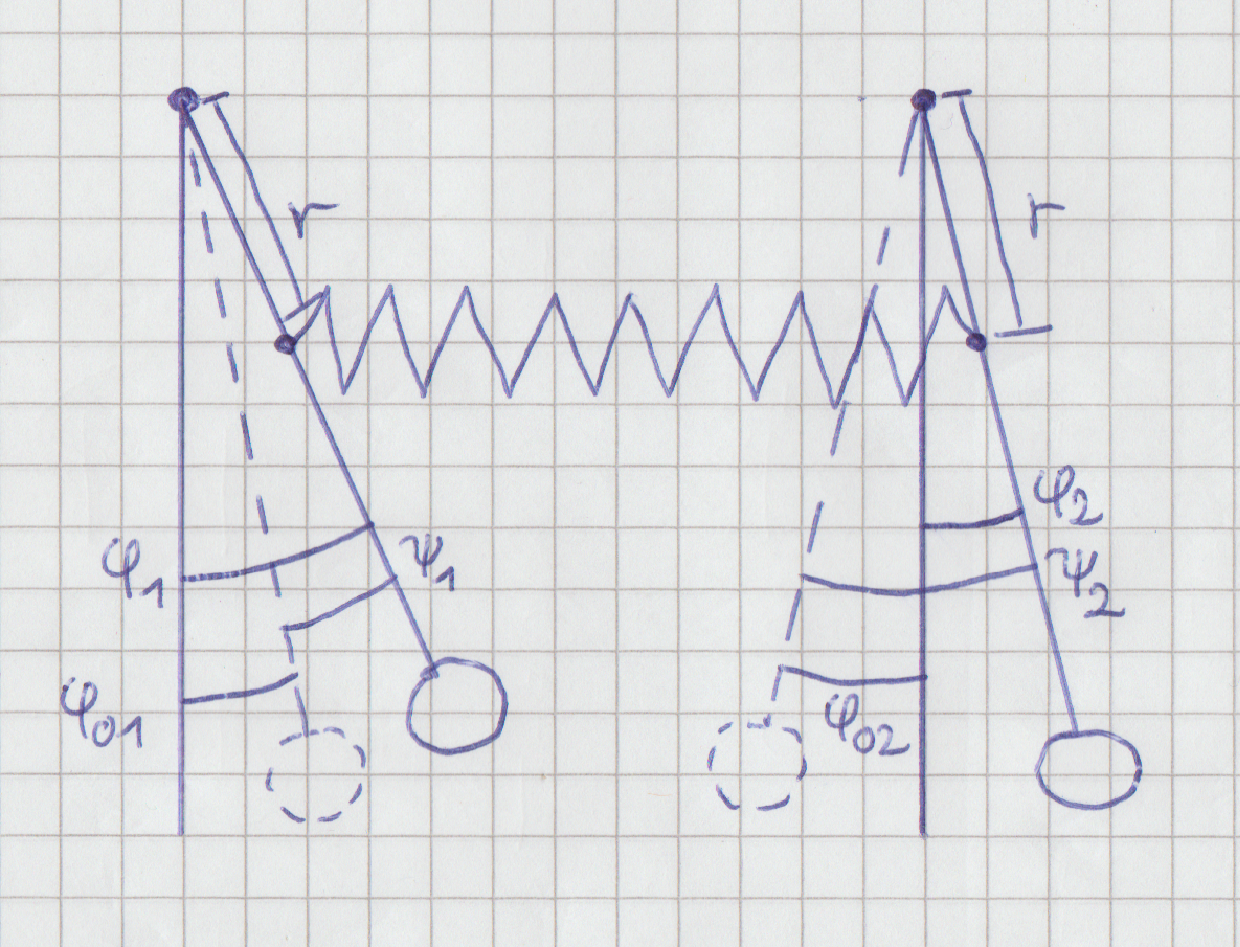
\includegraphics[width=0.7\textwidth]{./Bilder/gp}
\end{figure}
					\\
					Nun nutzen wir die Koordinatentransformation
					\begin{align*}
					\Psi_{1}:=\phi_{1}-\phi_{0}
					\end{align*}
					\begin{align*}
					\Psi_{2}:=\phi_{2}+\phi_{0}
					\end{align*}
					um vom Bezugssystem der Lotgeraden ins Bezugssystem der Ruhelagen der Pendel zu wechseln. Da in der Ruhelage keine Drehmomente existieren, ergibt sich durch kurze Umformung:
					\begin{align}
					M_{0}=(2Dr^{2}+\tilde{D})\cdot \phi_{0}
					\end{align} 
					Damit folgt dann 
					\begin{align}
					M_{1}=-\tilde{D}\cdot \Psi_{1}+Dr^{2}(\Psi_{2}-\Psi_{1})
					\end{align}
					\begin{align}
					M_{2}=-\tilde{D}\cdot \Psi_{2}-Dr^{2}(\Psi_{2}-\Psi_{1})
					\end{align}
					mit 
					\begin{align*}
					M_{1}=\Theta\cdot \ddot{\Psi_{1}}(t)
					\end{align*}
					\begin{align*}
					M_{2}=\Theta \cdot \ddot{\Psi_{2}}(t)
					\end{align*}
					\begin{align*}
					\omega_{gl}^{2}=\frac{\tilde{D}}{\Theta}
					\end{align*}
					\begin{align*}
					k^{2}=\frac{Dr^{2}}{\Theta}
					\end{align*}
					ergibt sich schließlich
					\begin{align}
					\ddot{\Psi_{1}}(t)+\omega_{gl}^{2}\cdot \Psi_{1}=k^{2}(\Psi_{2}-\Psi_{1})
					\end{align}
					\begin{align}
					\ddot{\Psi_{2}}(t)+\omega_{gl}^{2}\cdot \Psi_{2}=-k^{2}(\Psi_{2}-\Psi_{1})
					\end{align}
					Aus der Summe und der Differenz von (8) und (9) folgt
					\begin{align}
					\frac{d^{2}}{dt^{2}}(\Psi_{2}+\Psi_{1})+\omega_{gl}^{2}=0
					\end{align}
					\begin{align}
					\frac{d^{2}}{dt^{2}}(\Psi_{2}-\Psi_{1})+\omega_{gl}^{2}(\Psi_{2}-\Psi_{1})=-2k^{2}(\Psi_{2}-\Psi_{1})
					\end{align}
					mit der Substitution
					\begin{align*}
					m:=\Psi_{1}+\Psi_{2}
					\end{align*}
					\begin{align*}
					n:=\Psi_{1}-\Psi_{2}
					\end{align*}
					folgt
					\begin{align}
					\ddot{m}+\omega_{gl}^{2}\cdot m=0
					\end{align}
					\begin{align}
					\ddot{n}+(\omega_{gl}^{2}+2k^{2})\cdot n = 0
					\end{align}
					mit \(\omega_{gl}^{2}+2k^{2}=\omega_{geg}^{2}\)
					erhält man dann die allgemeine Lösungen:
					\begin{align}
					m(t)=a_{1}sin(\omega_{gl}t)+a_{2}cos(\omega_{gl}t)
					\end{align}
					\begin{align}
					n(t)=a_{3}sin(\omega_{geg}t)+a_{4}cos(\omega_{geg}t)
					\end{align}
					\newpage
					Die Lösungen für die \(\Psi(t)\) erhält man dann durch Rücktransformation mit \(\Psi_{1}(t)=\frac{m+n}{2}\) und \(\Psi_{2}(t)=\frac{m-n}{2}\) und die \(\phi(t)\) über \(\phi_{1}(t)=\Psi_{1}(t)+\phi_{0}\) und \(\phi_{2}(t)=\Psi_{2}(t)-\phi_{0}\). Der allgemeine Fall der gekoppelten Schwingung ist also eine Überlagerung der zwei Fundamentalschwingungen mit \(\omega_{gl}\) (Frequenz der gleichsinnig schwingenden Pendel) und \(\omega_{geg}\) (Frequenz der gegenphasig schwingenden Pendel). 
				\end{itemize}
			
			\end{itemize}
		\subsection{Schwingungsdauern}
			\begin{align}
			\omega_{gl}=\sqrt{\frac{g}{L}}
			\end{align}
			\begin{align}
			\omega_{geg}=\sqrt{\frac{g+2k}{L}}
			\end{align}
			Es ergeben sich die natürlichen Oszillationsperioden:
			\begin{align}
			T_{gl}=2\pi \sqrt{\frac{L}{g}}
			\end{align}
			\begin{align}
			T_{geg}=2\pi \sqrt{\frac{L}{g+2k}}
			\end{align}
			mit
			\begin{align*}
			\omega_{-}=\frac{\omega_{geg}-\omega_{gl}}{2}
			\end{align*}
			\begin{align*}
			\omega_{+}=\frac{\omega_{geg}+\omega_{gl}}{2}
			\end{align*}
			ergibt sich für die mittlere Periode einer gekoppelten Schwingung
			\begin{align}
			T_{m}=2\cdot \frac{T_{gl}\cdot T_{geg}}{T_{geg}+T_{gl}}
			\end{align}
			und für die Schwebungsdauer
			\begin{align}
			T_{S}=2\cdot \frac{T_{gl}\cdot T_{geg}}{T_{gl}-T_{geg}}
			\end{align}
		
		\subsection{Kopplungsgrad}
			Der Kopplungsgrad ist ein Maß für die Stärke der Kopplung.
			\begin{align}
			K:=\frac{\omega_{geg}^{2}-\omega_{gl}^{2}}{\omega_{geg}^{2}+\omega_{gl}^{2}}=\frac{T_{gl}^{2}-T_{geg}^{2}}{T_{gl}^{2}+T_{geg}^{2}}=\frac{Dr^{2}}{\tilde{D}+Dr^{2}}
			\end{align}
			
	\section{Fragen und Aufgaben zur Vorbereitung}
		\subsection{Aufgabe 1}
			Ist die Eigenkreisfrequenz \(\omega_{geg}\) bei gegenphasiger Schwingung kleiner, gleich oder größer als
			bei gleichsinniger Schwingung \(\omega_{gl}\)?\\
			\\
			Es gilt nach (16) und (17):
			\begin{align*}
			\omega_{gl}=\sqrt{\frac{g}{L}}
			\end{align*}
			\begin{align}
			\omega_{geg}=\sqrt{\frac{g+2k}{L}}
			\end{align}	
			daraus folgt offensichtlich \(\omega_{geg}>\omega_{gl}\)
			
		\subsection{Aufgabe 2}
			Welche Bedeutung haben gekoppelte Schwingungen in der Molekülphysik?\\
			\\
			Atome, die sich in Molekülen befinden können mit gekoppelten Pendeln verglichen werden, da die Atome um ihre Ruhelagen innerhalb des Moleküls oszillieren können. Die Bindungen zwischen den Atomen werden dabei als Federn betrachtet. Die Schwingungen der Atome um ihre jeweilige Ruhelage ist dabei abhängig von den Parametern Druck und Temperatur, sowie gegebenenfalls von der Anregung durch elektromagnetische Wellen. Somit bilden gekoppelte Pendel eine Möglichkeit, die Schwingungen der Atome näherungsweise zu beschreiben.
			
		\subsection{Aufgabe 3}
			Wie kann man Schwebungen zum Stimmen von Musikinstrumenten verwenden? Warum eignet
			sich diese Methode insbesondere bei tiefen Frequenzen? Wie kann man mit Schwebungen sehr
			hohe Frequenzen messen?\\
			\\
			Nimmt man ein Musikinstrument mit schwingenden Saiten, so kann man durch die Schwebungen erkennen, ob die Saiten gestimmt sind. Erzeugt man zwei Töne gleicher Lautstärke, so dass die Schwingungen die gleiche Amplitude besitzen, mit leicht verschiedenen Frequenzen, so nimmt ein menschliches Ohr nicht beide Töne getrennt wahr, sondern eine Art An- und Abschwellen eines Tones in der Höhe der Ausgangstöne. Das ist dann eine Schwebung. Wenn diese Schwebung hörbar ist, ist das Musikinstrument vermutlich nicht richtig gestimmt. Man kann es dann so stimmen, dass die Schwebung nicht mehr auftritt. Je tiefer ein Ton ist, desto tiefer ist auch seine Frequenz. Es gilt \(T=\frac{1}{f}\). Also ist \(T\) größer, bzw. länger, je kleiner, bzw. niedriger \(f\) ist. Somit folgt mit (21), dass die Schwebungsdauer für kleine Frequenzen größer ist, als für hohe. Da \(T_{S}\) also bei niedrigen Frequenzen länger ist, kann man sie besser hören und dadurch ist diese Stimmmethode vor allem bei tiefen Frequenzen geeignet.\\
			Man kann mit Hilfe der Schwebung aber auch sehr hohe Frequenzen messen, indem man einen Ton mit einer ähnlichen Frequenz generiert. Anhand der dabei auftretenden Schwebung und der dazugehörigen Schwebungsdauer kann man dann die Frequenz des ursprünglichen Tons ermitteln. Es  gilt \(T_{S}=\frac{2\pi}{\omega_{S}}\) wobei \(\omega_{S}=\frac{\omega_{1}-\omega_{2}}{2}\), da \(\omega_{2}\) bekannt ist, ergibt sich somit die gesuchte Frequenz durch \(\omega_{1}=2\omega_{S}+\omega_{2}\). 
			
		\subsection{Aufgabe 4}
			Wie kann mittels eines sog. FRAHMschen Schlingertanks die Schlingerbewegung eines großen
			Schiffs verringert werden (Schiffs-Stabilisator)?\\
			\\
			Wenn ein Schiff periodisch von Wellen in dessen Resonanzfrequenz getroffen wird, wird das hin- und herschaukeln des Schiffes größer und größer, was im Grunde genommen einer Resonanzkatastrophe entspricht. und im Extremfall das Schiff zum Kentern bringen kann. Das kann man mit Hilfe eines FRAHMschen Schlingertanks verhindern. Dabei handelt es sich um eine U-förmige Wassersäule, welche wiederum selbst im Schiff schwingt. Durch solche Tanks wird eine sekundäre Resonanz zusätzlich zu der äußeren der eintreffenden Wellen erzeugt, die der äußeren entgegenwirkt. So ist im Resonanzfall die Phase der Schwingung des Schiffs um \(90^{\circ}\) zu den äußeren Wellen verschoben. Das gleiche trifft auch auf die Wellen im Tank im Vergleich zu der Schwingung des Schiffes. Man hat also eine Phasenverschiebung von \(180^{\circ}\) zwischen den äußeren Wellen und denen im Tank. Somit heben sich diese gegenseitig auf und das Schwanken des Schiffes wird vermindert.
\end{document}